% HET IP section

%----------------------------------------------------------------
% Demonstration of convolution to fit iodine atlas
% plot made by ~/Exo.../HET.../plots_general/convol_kernel/deconv_plot.pro
\begin{figure}
\centering
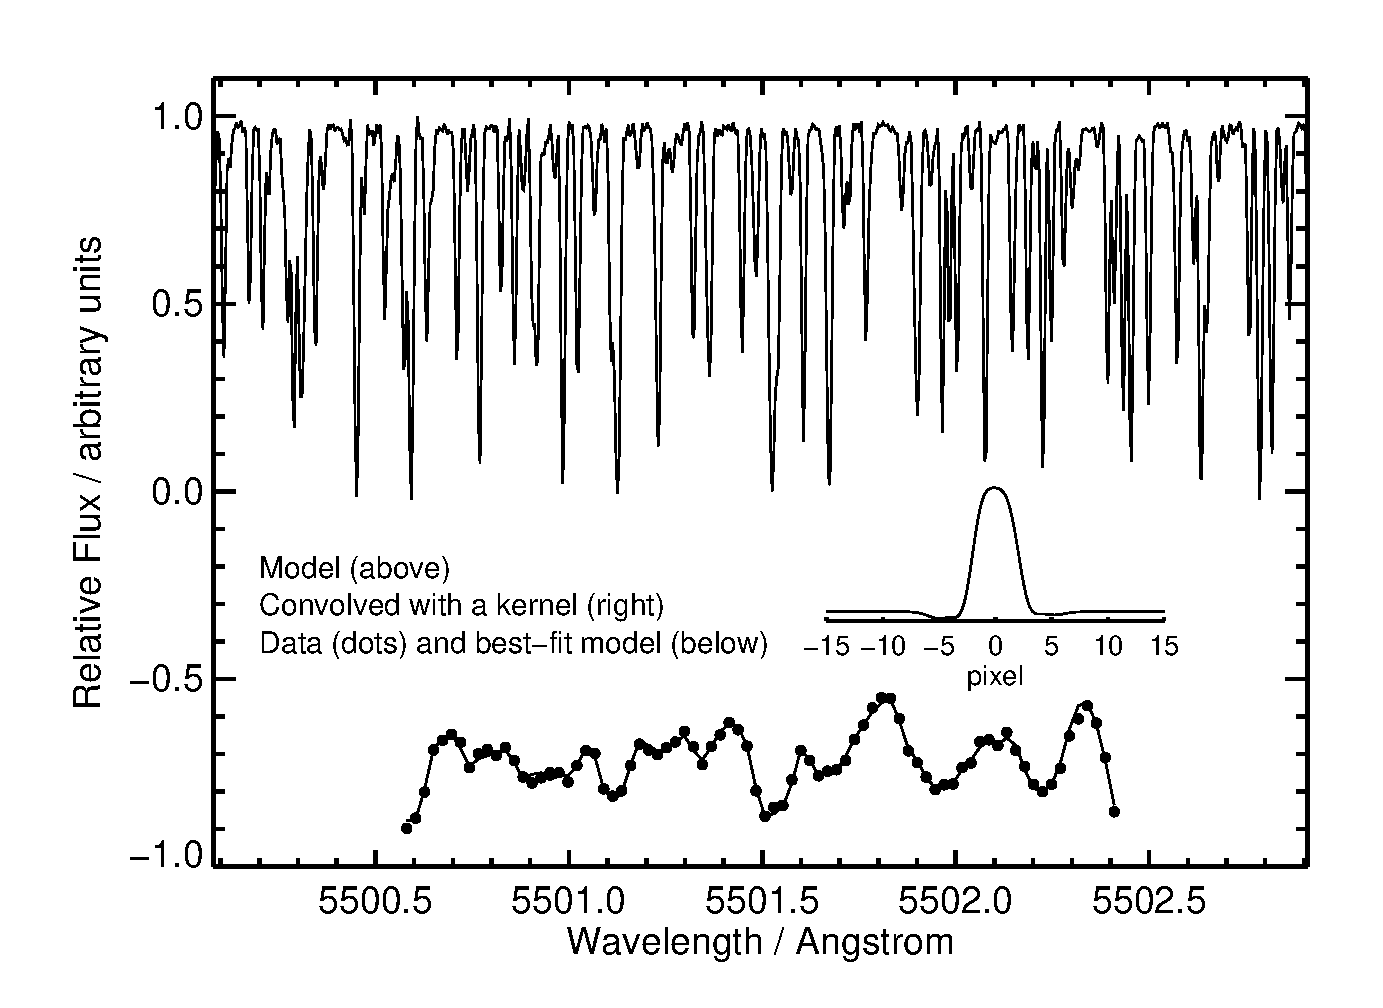
\includegraphics[scale=0.45]{het/convolution_kernel.eps}
\caption{Illustration of convolving the iodine atlas with a kernel to
  fit the observed iodine lines.
\label{het:fig:convkernel}}
\end{figure}
%----------------------------------------------------------------





%----------------------------------------------------------------
% Comparison between HET and Keck chunk fit
% plot made by ~/Exo.../HET.../plots_general/fit_demo/plotfit.pro
\begin{figure}
\centering
\subfloat[\het\ Chunk]{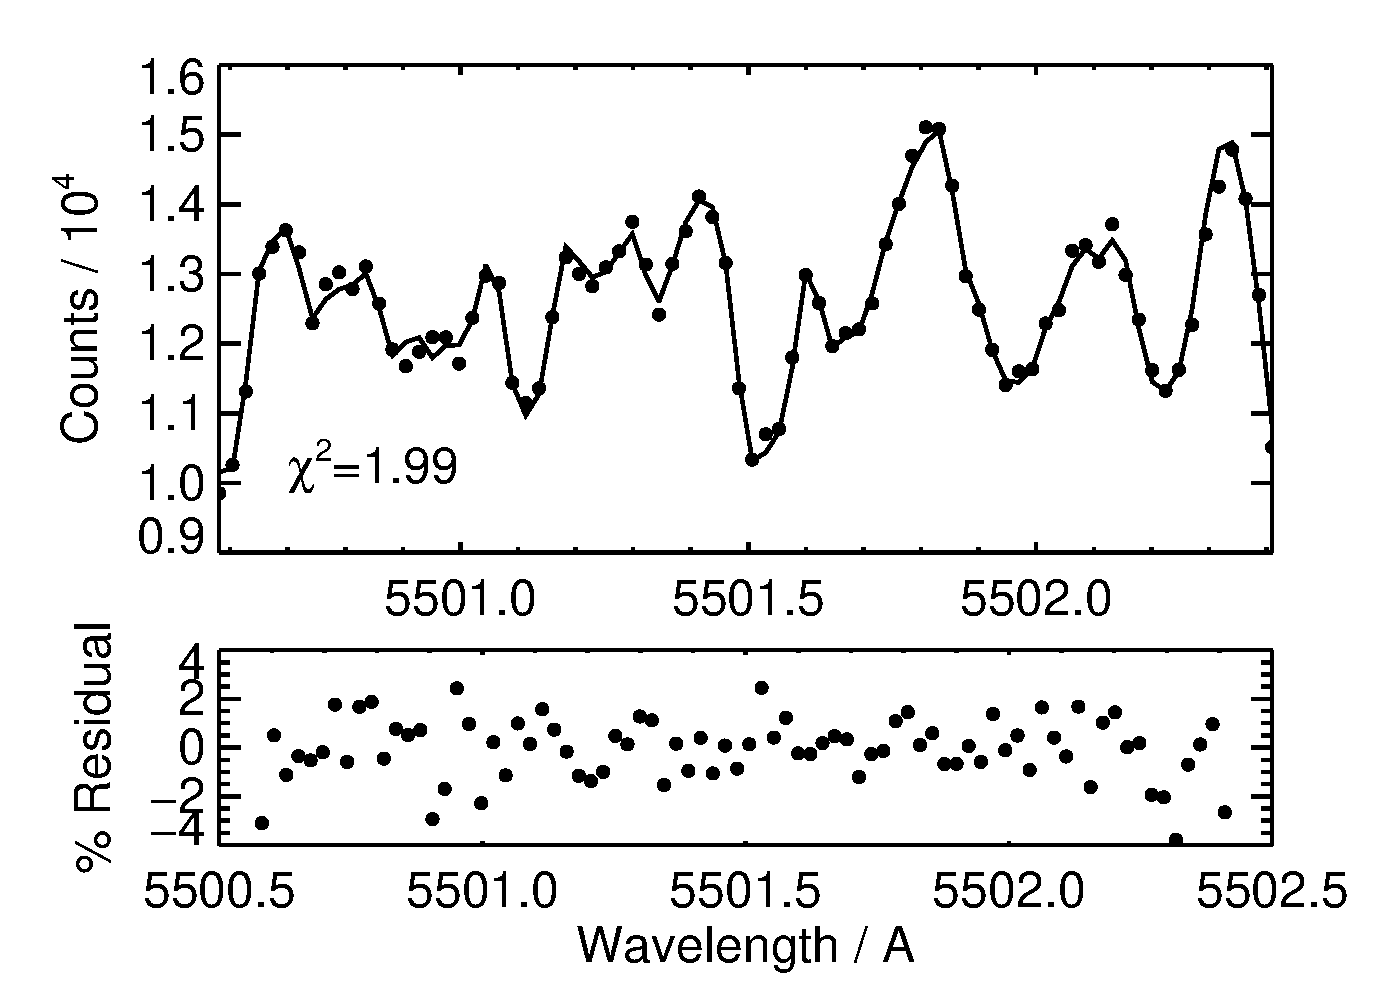
\includegraphics[scale=0.35]{het/20120124.176005.chunk189.eps}}
\subfloat[\keck\ Chunk]{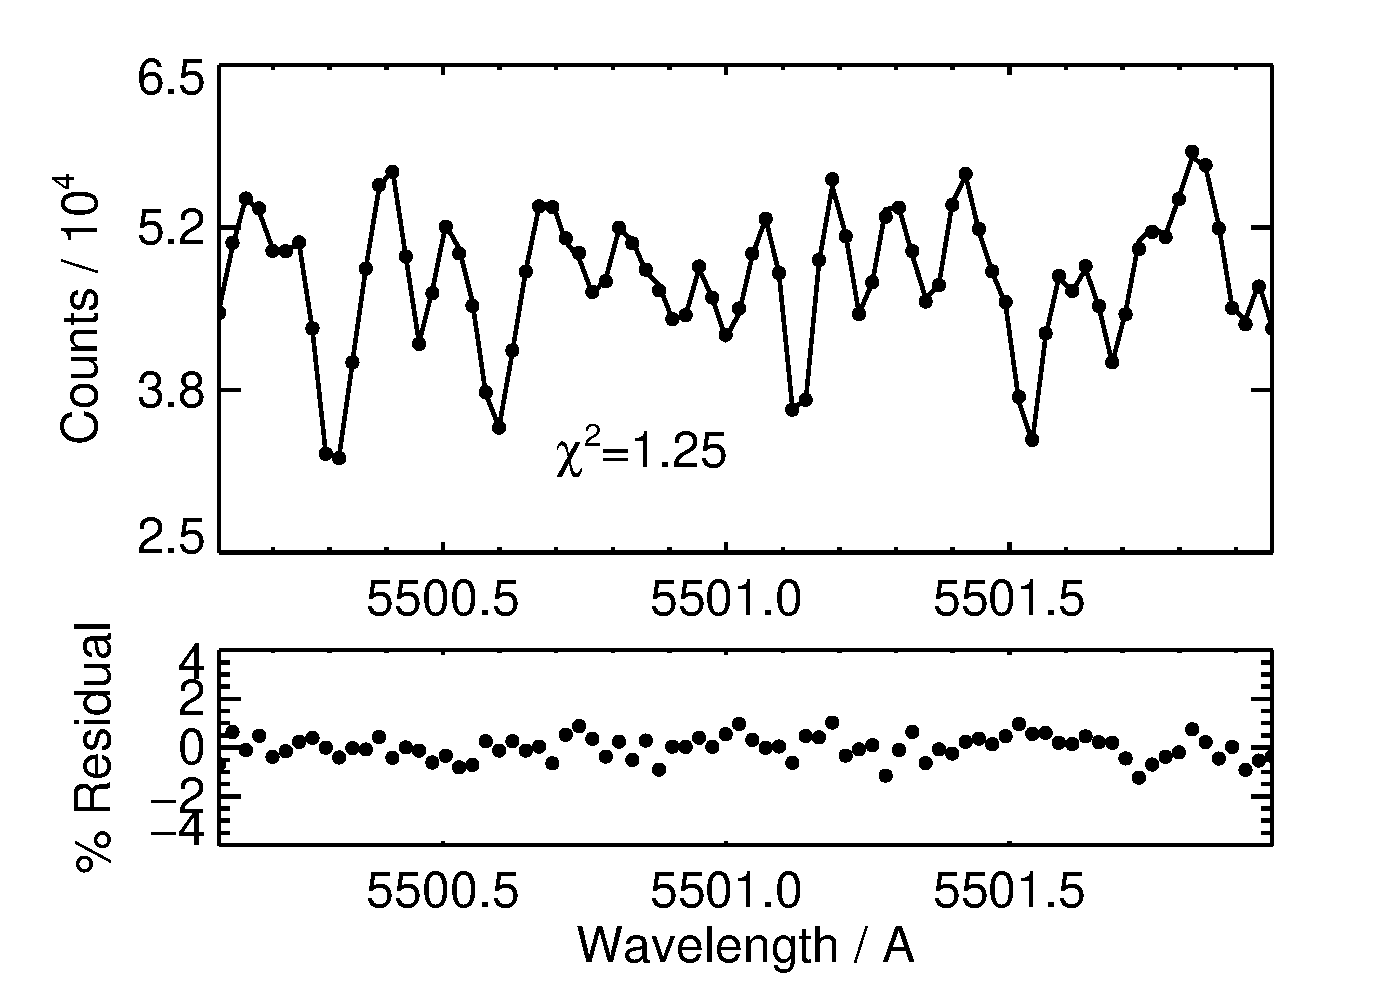
\includegraphics[scale=0.35]{het/rj82.77.chunk308.eps}}
\caption{
\label{het:fig:iodchunkcomp}}
\end{figure}
%----------------------------------------------------------------






%----------------------------------------------------------------
% Comparing 2005 and 2008 data, with GH and Gaussian IPs
% plot from ~/ExoPlanet-2010-2011/Professional_Development/201000-NSF_Jason/plots/
\begin{figure}
\centering
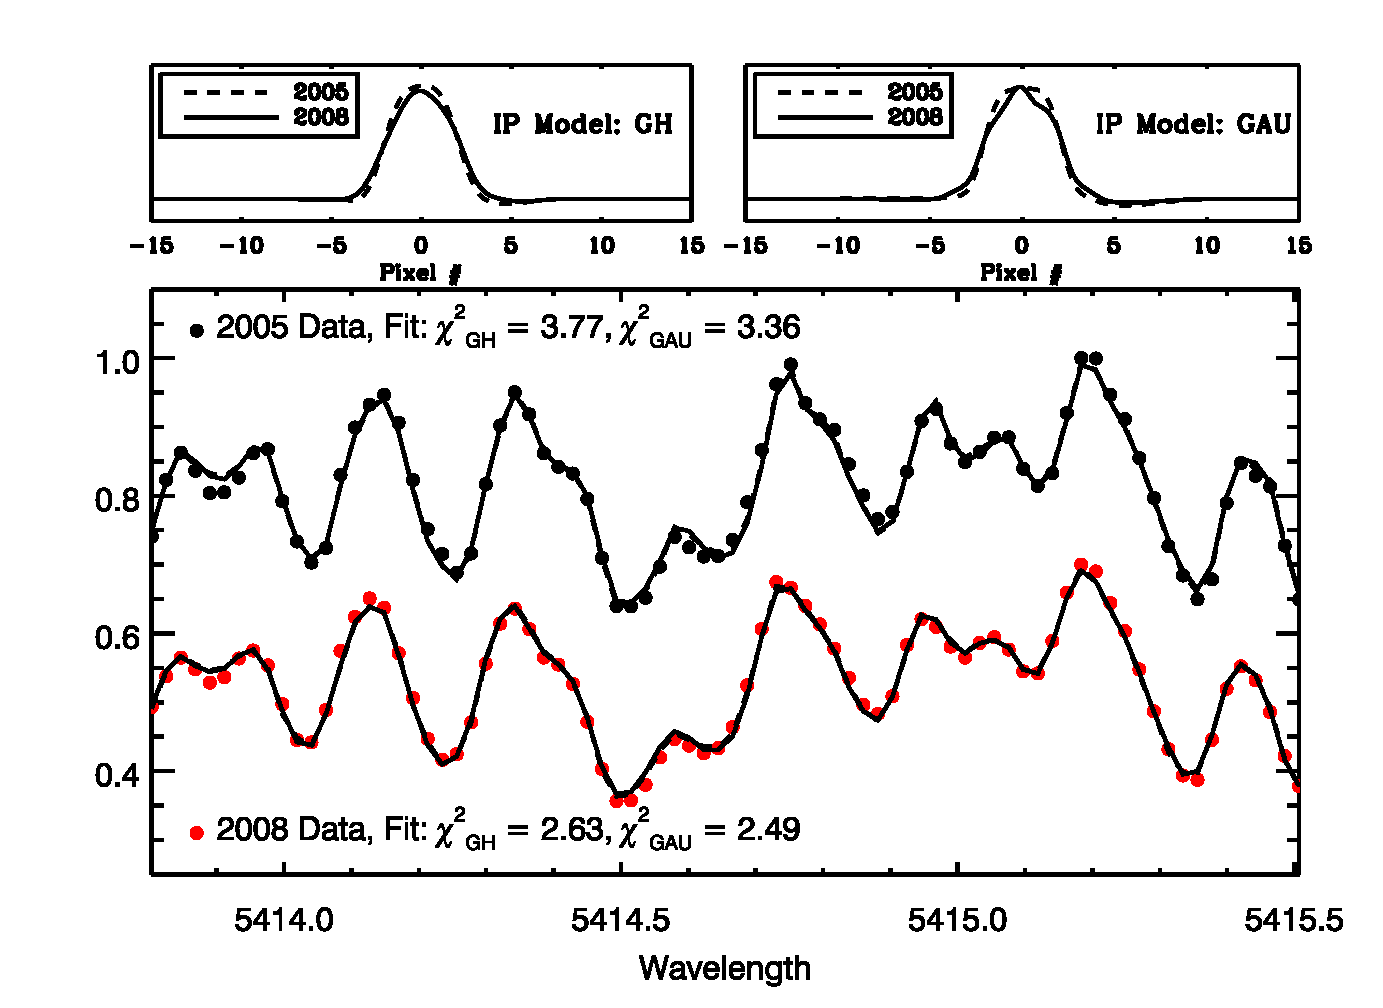
\includegraphics[scale=0.45]{het/iodfit.eps}
\caption{
\label{het:fig:ghgau}}
\end{figure}
%----------------------------------------------------------------




%----------------------------------------------------------------
% Comparing Keck and HET IPs in Fourier space
% plot from screen shot of a slide in
% ~/ExoPlanet-2010-2011/Professional_Development/20150727-ThesisCommMeet/
% original plot is from ~/Exo../HET.../06-line.../powspec.pro and stored in ./plots/
\begin{figure}
\centering
\includegraphics[scale=0.45]{het/fftip.eps}
\caption{Clear signature of \het\ slit (R $=$ 60k). A hint of \keck\
  slit too.
\label{het:fig:fftip}}
\end{figure}
%----------------------------------------------------------------



%----------------------------------------------------------------
% Fitting with a Moffat function
% plot made by ~/ExoPlanet-2010-2011/HET-HRS-IP/06-line_through_dots/thar.pro
% and stored in ./plots/
\begin{figure}
\centering
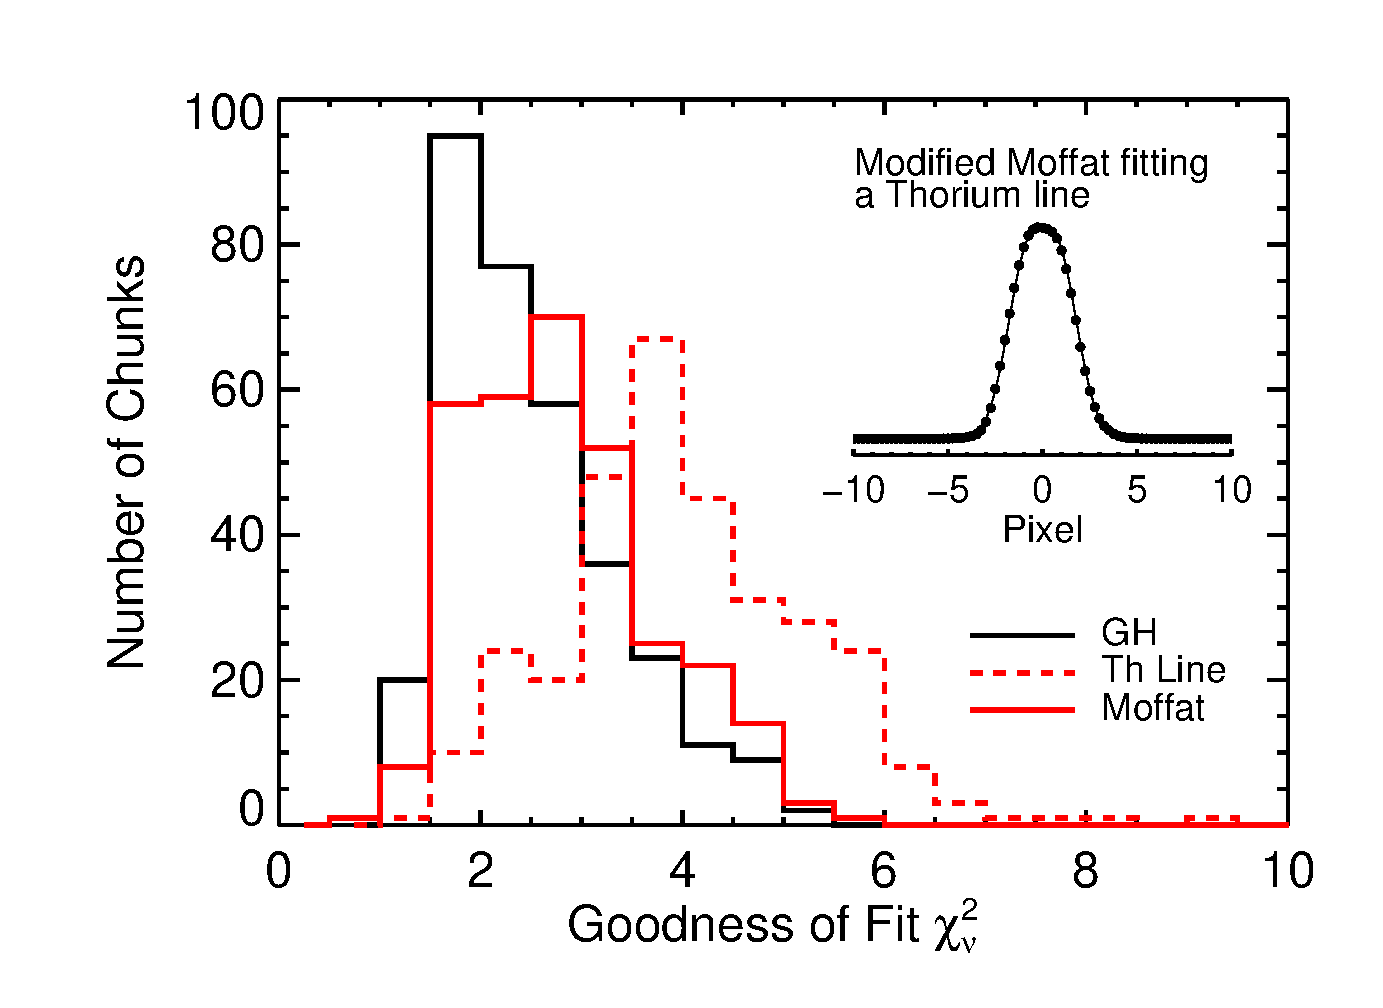
\includegraphics[scale=0.45]{het/thar_vs_moffat.eps}
\caption{
\label{het:fig:moffat}}
\end{figure}
%----------------------------------------------------------------





%----------------------------------------------------------------
% Comparing fits with two IPs
% plot made by ~/Exo.../HET.../plots_general/fit_demo/compfit.pro
\begin{figure}
\centering
\subfloat{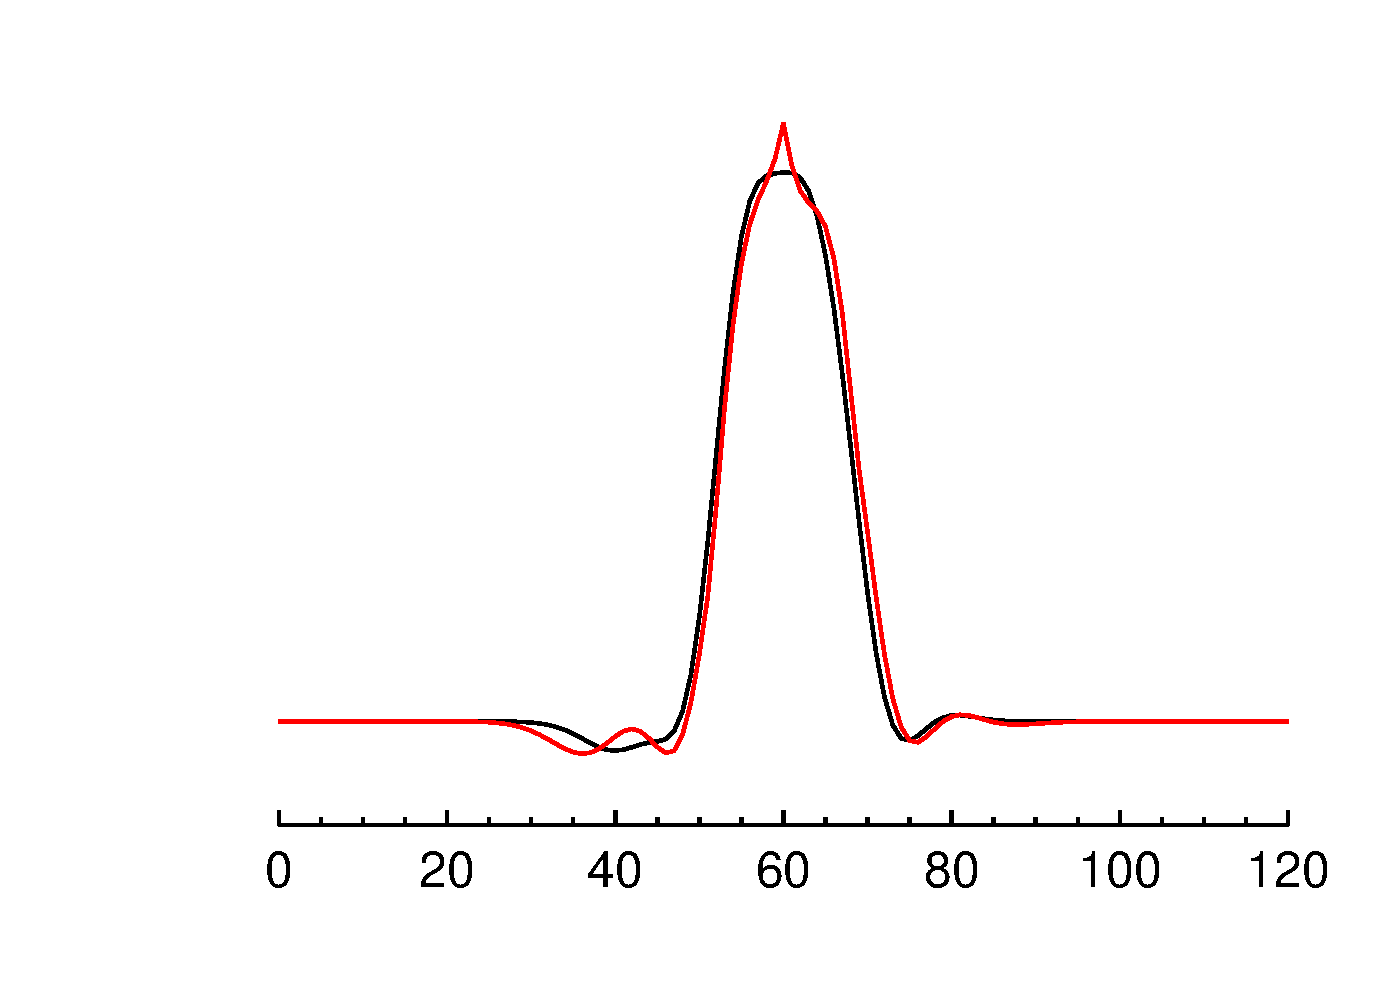
\includegraphics[scale=0.3]{het/20120124.176005.chunk191.compip.eps}}
\subfloat{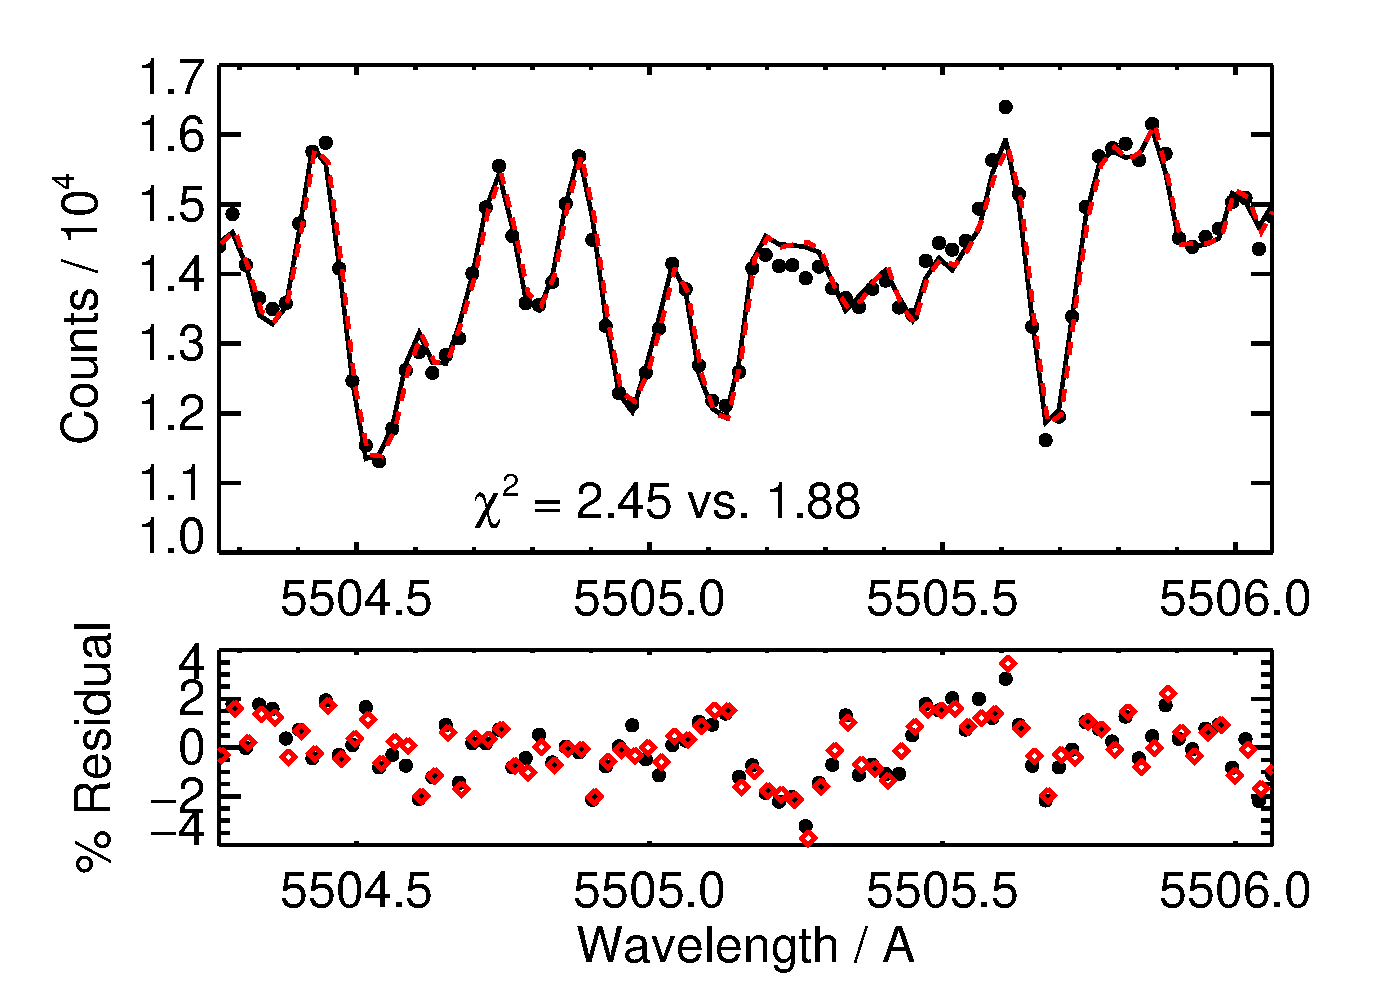
\includegraphics[scale=0.35]{het/20120124.176005.chunk191.compfit.eps}}
\caption{
\label{het:fig:iodipcomp}}
\end{figure}
%----------------------------------------------------------------

